% This is a Basic Assignment Paper but with like Code and stuff allowed in it, there is also url, hyperlinks from contents included. 

\documentclass[11pt]{article}

% Preamble

\usepackage[margin=1in]{geometry}
\usepackage{amsfonts, amsmath, amssymb}
\usepackage{fancyhdr, float, graphicx}
\usepackage[utf8]{inputenc} % Required for inputting international characters
\usepackage[T1]{fontenc} % Output font encoding for international characters
\usepackage{fouriernc} % Use the New Century Schoolbook font
\usepackage[nottoc, notlot, notlof]{tocbibind}
\usepackage{listings}
\usepackage{xcolor}
\usepackage{blindtext}
\usepackage{hyperref}
\hypersetup{
    colorlinks=true,
    linkcolor=black,
    filecolor=magenta,      
    urlcolor=cyan,
    pdfpagemode=FullScreen,
    }

\definecolor{codegreen}{rgb}{0,0.6,0}
\definecolor{codegray}{rgb}{0.5,0.5,0.5}
\definecolor{codepurple}{rgb}{0.58,0,0.82}
\definecolor{backcolour}{rgb}{0.95,0.95,0.92}

\lstdefinestyle{mystyle}{
    backgroundcolor=\color{backcolour},   
    commentstyle=\color{codegreen},
    keywordstyle=\color{magenta},
    numberstyle=\tiny\color{codegray},
    stringstyle=\color{codepurple},
    basicstyle=\ttfamily\footnotesize,
    breakatwhitespace=false,         
    breaklines=true,                 
    captionpos=b,                    
    keepspaces=true,                 
    numbers=left,                    
    numbersep=5pt,                  
    showspaces=false,                
    showstringspaces=false,
    showtabs=false,                  
    tabsize=2
}

\lstset{style=mystyle}

% Header and Footer
\pagestyle{fancy}
\fancyhead{}
\fancyfoot{}
\fancyhead[L]{\textit{\Large{SRS for Attendance Assistant}}}
%\fancyhead[R]{\textit{something}}
\fancyfoot[C]{\thepage}
\renewcommand{\footrulewidth}{1pt}



% Other Doc Editing
% \parindent 0ex
%\renewcommand{\baselinestretch}{1.5}

\begin{document}

\begin{titlepage}
	\centering

	%---------------------------NAMES-------------------------------

	\huge\textsc{
		MIT World Peace University
	}\\

	\vspace{0.75\baselineskip} % space after Uni Name

	\LARGE{
		Software Engineering and Testing\\
		Second Year B. Tech, Semester 4
	}

	\vfill % space after Sub Name

	%--------------------------TITLE-------------------------------

	\rule{\textwidth}{1.6pt}\vspace*{-\baselineskip}\vspace*{2pt}
	\rule{\textwidth}{0.6pt}
	\vspace{0.75\baselineskip} % Whitespace above the title



	\huge{\textsc{
			Performing Secure Systems\\ Analysis And Design \\
			Drawing Data Flow Diagrams (Level 0, 1, 2)
		}} \\



	\vspace{0.5\baselineskip} % Whitespace below the title
	\rule{\textwidth}{0.6pt}\vspace*{-\baselineskip}\vspace*{2.8pt}
	\rule{\textwidth}{1.6pt}

	\vspace{1\baselineskip} % Whitespace after the title block

	%--------------------------SUBTITLE --------------------------	

	\LARGE\textsc{
		Assignment 2
	} % Subtitle or further description
	\vfill

	%--------------------------AUTHOR-------------------------------

	Prepared By
	\vspace{0.5\baselineskip} % Whitespace before the editors

	\Large{
		Krishnaraj Thadesar \\
		Cyber Security and Forensics\\
		Batch A1, PA 20
	}


	\vspace{0.5\baselineskip} % Whitespace below the editor list
	\today

\end{titlepage}


\tableofcontents
\thispagestyle{empty}
\clearpage

\setcounter{page}{1}

\section{Aim}
Aim: Perform the Structured Systems Analysis and Design (SSAD) - Draw the DFD MODEL
(Level 0, Level 1 and Level 2). Use an open source tool for the same.


\section{Objectives}

\begin{enumerate}
	\item To understand the different levels of DFD in Library management system.
	\item To choose and use levels DFD .
	\item To learn and understand the different concept structured system design.
\end{enumerate}

\section{Problem Statement}

\textbf{Draw DFD of level 0, level 1 and level 2 for The Following Problem:} \\

\textit{The Purpose of an Attandence Assistant App is to help reduce the time taken for recording the attendance of a classroom in a school or college. The app will be able to record the attendance of a class in a matter of a few Seconds with minimum Energy Expended. It will record data on cloud, and be accessible to all the Teachers.}\\

\section{Theory}

\subsection{Data flow diagrams}
Data flow diagrams are used to describe data flow within a system. They can depict transformations on
data as well as storage locations. They trace the route that data travels in a system, from start to finish.

\subsection{Symbols Used (Yourdon and Coad)}
\begin{enumerate}

	\item External Entity : An external entity, which are also known as terminators, sources, sinks, or actors, are an outside system or process that sends or receives data to and from the diagrammed system. They’re either the sources or destinations of information, so they’re usually placed on the diagram’s edges.
	\item Process: Process is a procedure that manipulates the data and its flow by taking incoming data, changing it, and producing an output with it. A process can do this by performing computations and using logic to sort the data or change its flow of direction.
	\item Data Store: Data stores hold information for later use, like a file of documents that’s waiting to be processed. Data inputs flow through a process and then through a data store while data outputs flow out of a data store and then through a process.
	\item Data flow: Data flow is the path the system’s information takes from external entities through processes and data stores. With arrows and succinct labels, the DFD can show you the direction of the data flow.
\end{enumerate}

\subsection{Rules of DFD}
\begin{enumerate}
	\item Each process should have at least one input and one output.
	\item Each data store should have at least one data flow in and data flow out.
	\item A system’s stored data must go through a process.
	\item All processes in a DFD must link to another process or data store.
\end{enumerate}

\subsection{DFD Level 0, 1, 2}

Data flow diagrams are also categorized by level. Starting with the most basic, level 0, DFDs get
increasingly complex as the level increases.

\subsubsection{Level 0 DFDs}
Also known as context diagrams, are the most basic data flow diagrams. They provide abroad view that offers little detail. Level 0 data flow diagrams show a single process node and its
connections to external entities.

\subsubsection{Level 1 DFDs}
Level 1 DFDs are still a general overview, but they go into more detail than a context diagram. In a level
1 data flow diagram, the single process node from the context diagram is broken down into sub
processes.

\subsubsection{Level 2 DFDs}
Level 2+ DFDs simply break processes down into more detailed sub processes. Level 3 data flow
diagrams are detailed enough that it doesn't usually make sense to break them down further.

\section{Difference between DFD and CFD}
\begin{table}[H]
	\begin{tabular}{|l|l|}
		\hline
		Data Flow Diagram                                                                                                                                                                           & Control Flow Diagram                                                                                                       \\ \hline
		\begin{tabular}[c]{@{}l@{}}1. A data flow diagram (DFD) is a graphical \\ representation of the "flow"\\ of data through aninformation \\ system, modeling its process aspects\end{tabular} & \begin{tabular}[c]{@{}l@{}}1. It describe the control flow \\ of a businessprocess, process or program.\end{tabular}       \\ \hline
		\begin{tabular}[c]{@{}l@{}}2. It contains external entity, \\ process and data dictionary\end{tabular}                                                                                      & \begin{tabular}[c]{@{}l@{}}2. It contains Control Specification \\ (CSPEC) and Process Specification (PSPEC).\end{tabular} \\ \hline
		\begin{tabular}[c]{@{}l@{}}3. It contains various levels\\  like level 0, level 1 etc\end{tabular}                                                                                          & 3. There is no such levels like DFD.                                                                                       \\ \hline
		\begin{tabular}[c]{@{}l@{}}4. It will give idea about how \\ data will passed and how\\  output will be generated.\end{tabular}                                                             & \begin{tabular}[c]{@{}l@{}}4. To indicate How the software \\ behaves when an event is sensed.\end{tabular}                \\ \hline
	\end{tabular}
\end{table}

\section{Tables Generated}

\subsection{Students}

\begin{table}[H]
	\begin{tabular}{|l|l|l|l|l|}
		\hline
		\textbf{Sr. No } & \textbf{Name of the Student } & \textbf{Face of the Student                               } & \textbf{Roll Number} & \textbf{PRN of the student } \\ \hline
		1                & Krishnaraj Thadesar           & \textless{}face\_data\_from\_opencv\textgreater{}           & 20                                   & 1032210888                   \\ \hline
		2                & Devanshu Surana               & \textless{}face\_data\_from\_opencv\textgreater{}           & 37                                   & 1032201654                   \\ \hline
		3                & Parth Zarekar                 & \textless{}face\_data\_from\_opencv\textgreater{}           & 15                                   & 1032210846                   \\ \hline
		4                & Rohit Jobish                  & \textless{}face\_data\_from\_opencv\textgreater{}           & 89                                   & 1032210658                   \\ \hline
	\end{tabular}
\end{table}

\subsection{Classes}

\begin{table}[H]
	\begin{tabular}{|l|l|l|l|l|l|l|}
		\hline
		\textbf{Class ID } & \textbf{School } & \textbf{Section  } & \textbf{Panel } \\ \hline
		1001               & SCET             & CSE                & A               \\ \hline
		1002               & SCET             & CSF                & A               \\ \hline
		1003               & SCME             & Robotics           & A               \\ \hline
	\end{tabular}
\end{table}

\subsection{Programs}

\begin{table}[H]
	\begin{tabular}{|l|l|l|l|}
		\hline
		\textbf{P. No } & \textbf{School } & \textbf{Program Name                       } & \textbf{Number of  Panels } \\ \hline
		1               & SCET             & Computer Science and CyberSecurity           & 1                           \\ \hline
		2               & SCET             & CSE Artificial Intelligence and DS           & 2                           \\ \hline
	\end{tabular}
\end{table}

\subsection{Professors}
\begin{table}[H]
	\begin{tabular}{|l|l|l|l|}
		\hline
		\textbf{Professor ID } & \textbf{School } & \textbf{Subjets Taught } & \textbf{Name of Professor } \\ \hline
		1001                   & SCET             & CN                       & Lalit Kulkarni              \\ \hline
		1002                   & SCET             & {[}OS, SET{]}            & Jyoti Gavhane               \\ \hline
	\end{tabular}
\end{table}
\subsection{Subjects}

\begin{table}[H]
	\begin{tabular}{|l|l|l|l|}
		\hline
		\textbf{Professor ID } & \textbf{School } & \textbf{Subjets Taught } & \textbf{Name of Professor } \\ \hline
		1001                   & SCET             & CN                       & Lalit Kulkarni              \\ \hline
		1002                   & SCET             & {[}OS, SET{]}            & Jyoti Gavhane               \\ \hline
	\end{tabular}
\end{table}

\subsection{Attendance}

\begin{table}[H]
	\begin{tabular}{|l|l|l|l|l|}
		\hline
		\textbf{A.ID } & \textbf{Date      } & \textbf{Subject Name                     } & \textbf{PRN of Present Students}                                                                            & \textbf{PRN of Absent Students}      \\ \hline
		1              & 25/2/2023           & SET        & \begin{tabular}[c]{@{}l@{}}{[}1032210888, \\ 1032210553,\\ 1032210937,\\ ........1032210432{]}\end{tabular} & {[}1032133234, 122312345{]} \\ \hline
		2              & 25/2/2023           & ADS                   & \begin{tabular}[c]{@{}l@{}}{[}1032210888, \\ 1032210553,\\ 1032210937,\\ ........1032210432{]}\end{tabular} & {[}1032133234, 122312345{]} \\ \hline
	\end{tabular}
\end{table}


\section{Data Flow Diagram Level 0}
\begin{figure}[H]
    \begin{small}
        \begin{center}
            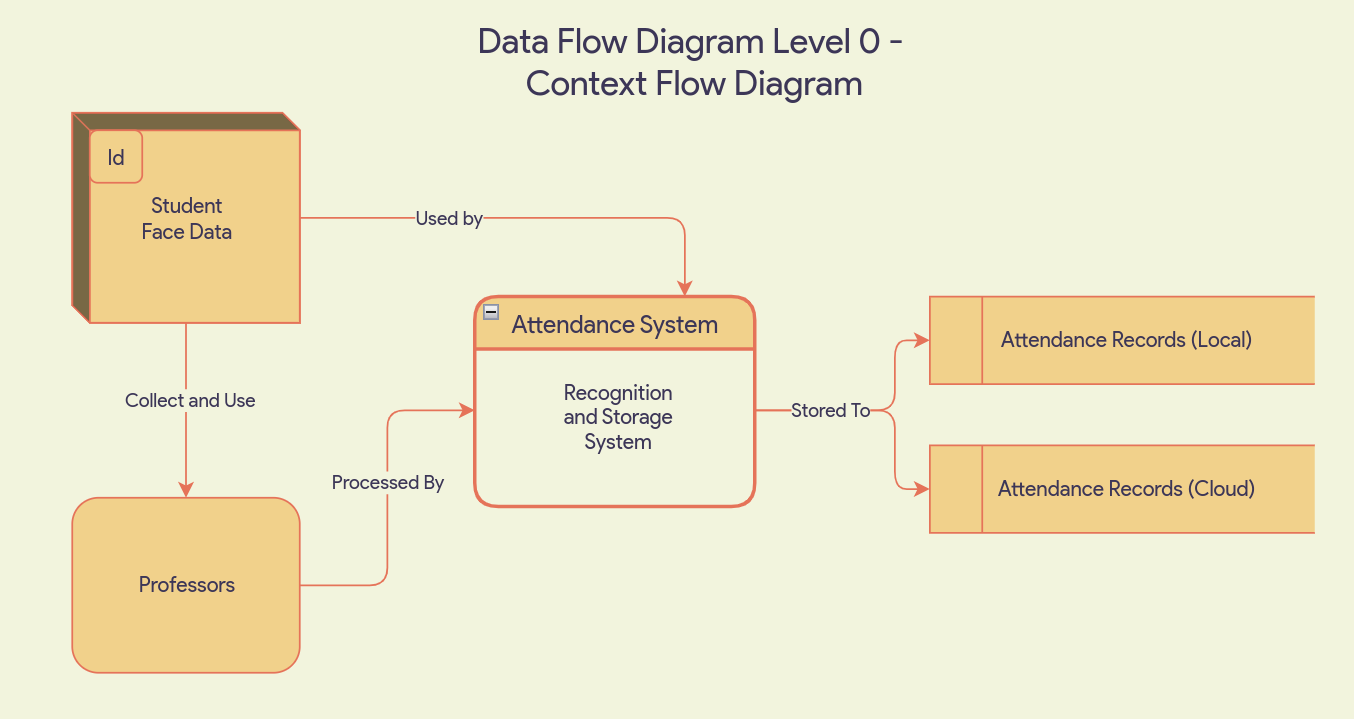
\includegraphics[scale=0.4]{dfd level 0.png}
        \end{center}
        \caption{}
        \label{fig:}
    \end{small}
\end{figure}

\section{Data Flow Diagram Level 1}

\begin{figure}[H]
    \begin{small}
        \begin{center}
            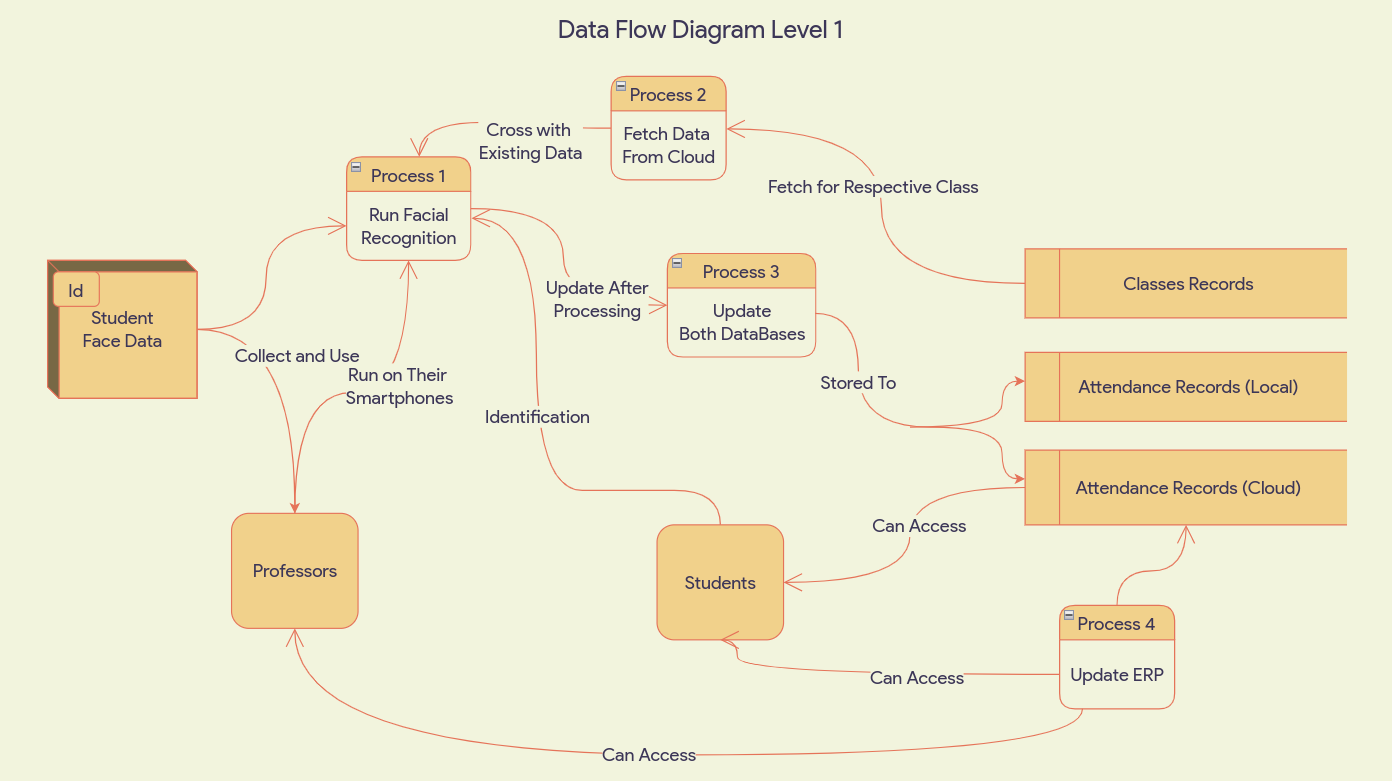
\includegraphics[scale=0.45]{dfd level 1.png}
        \end{center}
        \caption{}
        \label{fig:}
    \end{small}
\end{figure}


\section{Data Flow Diagram Level 2}

\begin{figure}[H]
    \begin{small}
        \begin{center}
            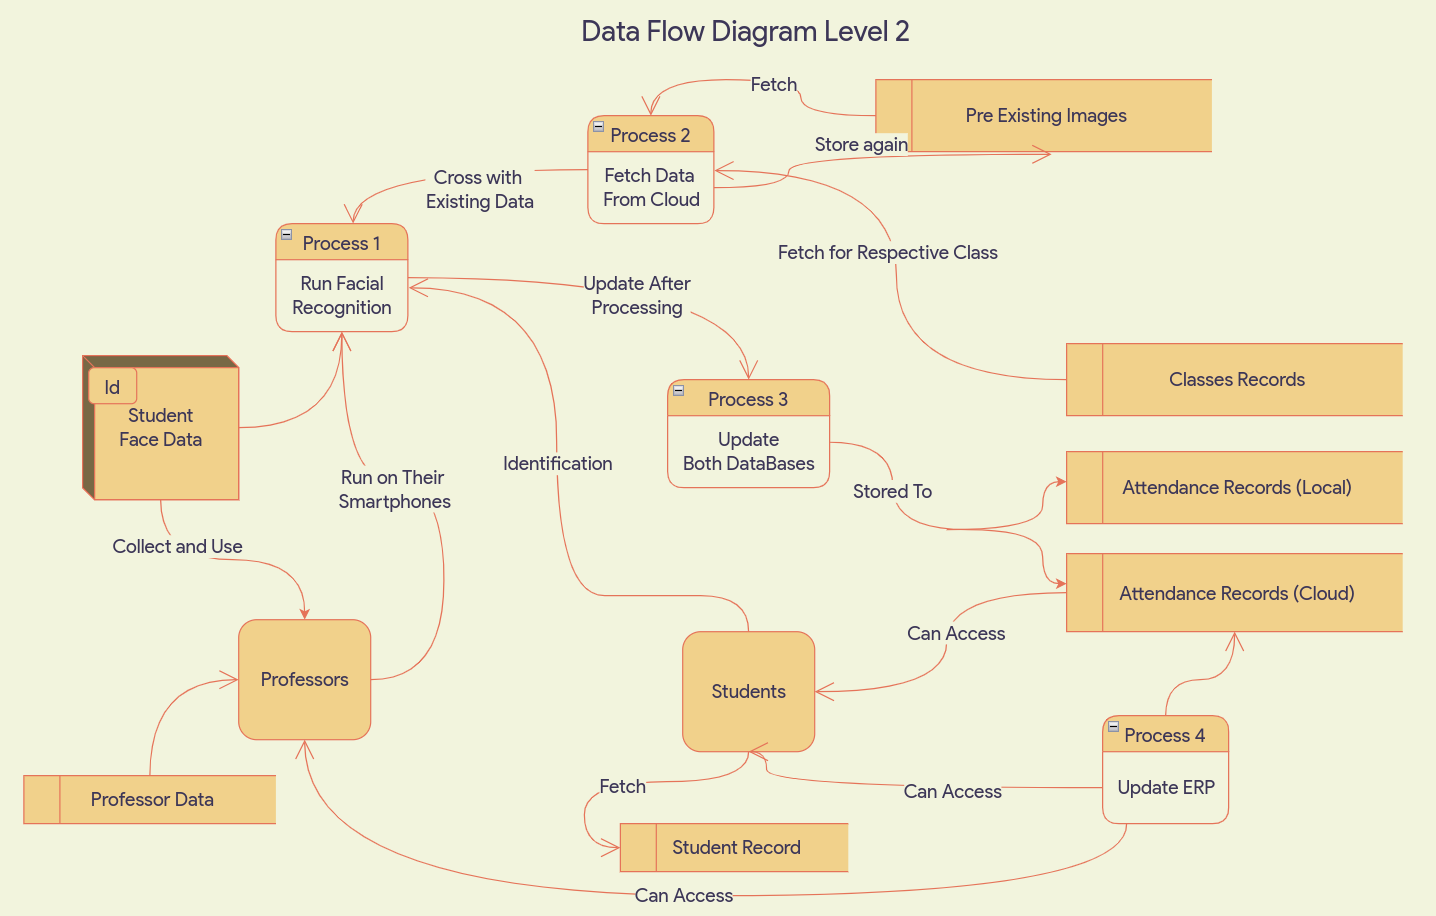
\includegraphics[scale=0.45]{dfd level 2.png}
        \end{center}
        \caption{}
        \label{fig:}
    \end{small}
\end{figure}


\section{Conclusion}
Hence, learned to draw data flow diagram of level 0, level 1 ,level 2 and control flow
diagram.

\section{FAQ}

\begin{enumerate}
	\item What is meant by context diagram?\\
	DFD Level 0 is also called a Context Diagram. It's a basic overview of the whole system or process being analyzed or modeled. It's designed to be an at-a-glance view, showing the system as a single high-level process, with its relationship to external entities. It should be easily understood by a wide audience, including stakeholders, business analysts, data analysts and developers. 

	\item What are different levels of Data flow diagram?\\
	
	A data flow diagram can dive into progressively more detail by using levels and layers, zeroing in on a particular piece.  DFD levels are numbered 0, 1 or 2, and occasionally go to even Level 3 or beyond. The necessary level of detail depends on the scope of what you are trying to accomplish. Level 0 is just a basic overview, Level 1 is a more detailed view, and Level 2 is the most detailed view.
	
	\item What are the data stored in the context diagram of problem Statement?\\
	The Context Diagram of Problem Statement contains the following data:

\end{enumerate}

\end{document}